\section{Roterende legemer}
Legemers bevægelse kan, i den Newtonske mekanik, deles op i to kategorier - translatorisk og rotationel bevægelse. Her menes bevægelse med og uden rotation. Vi starter med at se på den rotationelle del af legemers bevægelse, hvor der vil fokuseres på stive legemer, hvilket vil sige faste objekter, der ikke kan bøje eller deformeres. Beskrivelsen af legemers bevægelse deles op i tre dele - kinematik, energi og dynamik. Kinematik er beskrivelsen af legemers bevægelse, når bevægelsens oprindelse ikke tages med i betragtning. Dynamik beskriver hvorfor ting bevæger sig som de gør, og hvordan kinematiske bevægelser opstår. Det viser sig at energi er en vigtig størrelse at undersøge, når man skal beskrive bevægelse, hvorfor vi vil kigge på energien i både translatorisk og rotationel bevægelse.

\subsection{Kinematik}
I den translatoriske bevægelse beskrives et legemes position med en stedvektor $\va{r}$, der kan udtrykkes i forskellige koordinatsystemer. I det kartesiske koordinatsystem ser vektoren ud på en af følgende måder
%
\begin{align*}
	\va{r} = \begin{pmatrix}x \\ y \\ z \end{pmatrix} = x\vu{x} + y\vu{y} + z\vu{z} \: ,
\end{align*}
%
hvilket betyder at legemet befinder sig i punktet $(x,y,z)$. Ud fra stedvektoren defineres hastighed $\va{v}$ og acceleration $\va{a}$ som\footnote{Man kan selvfølgelig differentiere stedvektoren ligeså mange gange man lyster, og selvom højere afledede bruges meget sjældent, har de faktisk nogle navne (på engelsk), som man kan underholde sig selv ved at google. Den tredjeafledede $\dv*[3]{\va{r}}{t}$ er dog værd at fremhæve, da den på engelsk hedder "jerk".}
\begin{equation}
    \va{v} \equiv \dot{\va{r}} \: , \qquad \va{a} \equiv \ddot{\va{r}}.
\end{equation}
%
\begin{figure}[h!]
\centering
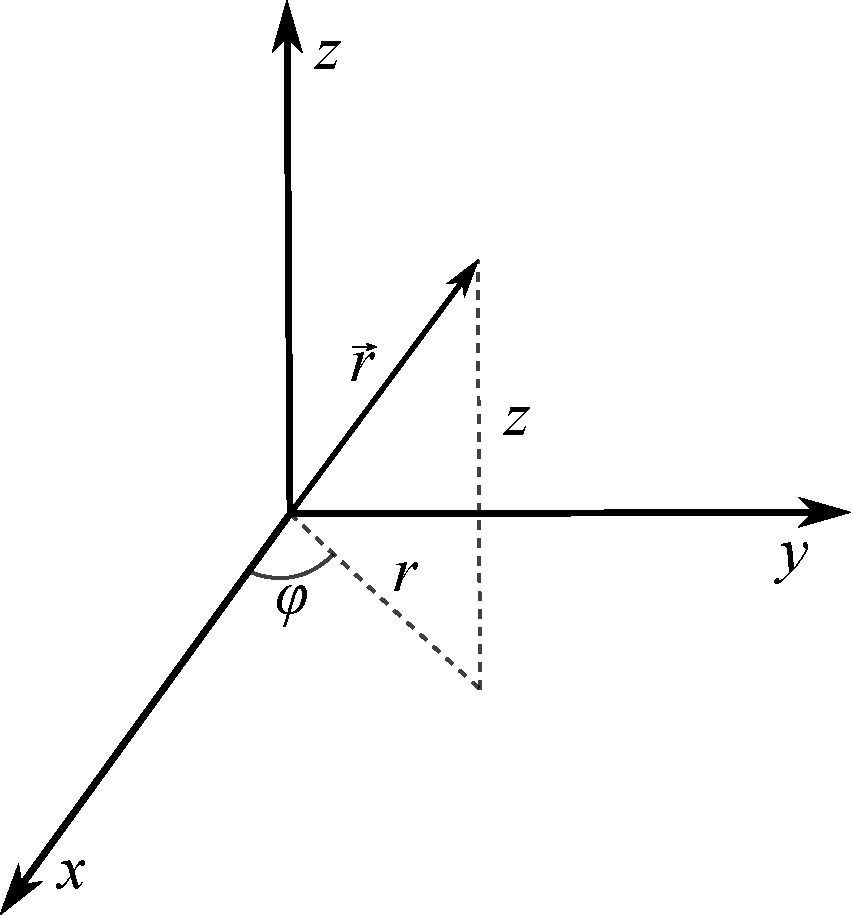
\includegraphics[width=.4\textwidth]{figurer/CylindriskeKoordinater}
\caption{I det cylindriske koordinatsystem angives afstanden til $z$-aksen som første koordinat, samt forskydningen langs samme akse som $z$-koordinat. Derudover angives vinklen med polæraksen, her ækvivalent med $x$-aksen. $z$-koordinatet er derved det samme i det kartesiske og cylindriske koordinatsystem.}
\label{mek:fig:CylindriskeKoordinater}
\end{figure}
%
%
\subsubsection{Cylindrisk polære koordinater}
Til beskrivelsen af roterende legemer benyttes ofte cylindriske koordinater i stedet for kartesiske koordinater. Cylindriske koordinater er en tredimensionel udvidelse af de todimensionelle polære koordinater, hvor 3. koordinatet, $z$, forskyder punktet parallelt med en akse, der er ortogonal (vinkelret) på den todimensionelle plan udspændt af de polære koordinater, gennem origo, (0,0,0). I polære koordinater defineres et punkt  som origo, og ud fra det en polærakse, der angiver placeringen af vinklen på $\phi = 0$ radianer. Et punkts afstand til origo, $r$, og dets vinkel med polæraksen, $\phi$, angiver så de polære koordinater. Defineres koordinatsystemet således at polæraksen og $x$-aksen i et tilsvarende kartesisk koordinatsystem er sammenfaldende, ville $\phi$ være vinklen ift. $x$-aksen i $xy$-planen og $z$ er forskydningen ift. polærplanen, se \cref{mek:fig:CylindriskeKoordinater}. Det bemærkes, at det kartesiske 3. koordinat og det cylindriske 3. koordinat er ens, og at afstanden $r$ ved udvidelsen fra polære til cylindriske koordinater forbliver uændret; det vil sige at en ændring i $z$ ikke giver en ændring i $r$. Da der kun fokuseres på legemers rotation om én akse, kan $z$-aksen defineres til at være denne rotationsakse, hvorved det cylindriske 3. koordinat forbliver uændret i tid.  \\

I polære koordinater er der en meget nyttig sammenhæng mellem et legemes totale fart og den tidsafledte af vinkelkoordinatet $\dot{\phi}$. Det antages at førstekoordinatet, $r$, er konstant i tid, $\dot{r} = 0$. Derfor kan \cref{mek:eq:kartesisk/polaer} fra matematikafsnittet\footnote{I matematikafsnittet hedder vinklen $\theta$, hvor den her hedder $\phi$. Det betyder ikke det store hvad man kalder den, men her i kapitlet bruges $\phi$, hvor denne notation bruges konsekvent.} benyttes til at opskrive de tidsafledede af de kartesiske koordinater udtrykt ved de polære koordinater
%
\begin{equation}
\begin{aligned}
	\dot{x} &= -r\sin\phi\dot{\phi} \: , \\
	\dot{y} &= r\cos\phi\dot{\phi} \: .
\end{aligned}
\end{equation}
%
Da hastighed er en vektor, $\va{v} = \dot{x} \vu{x} + \dot{y} \vu{y}$, så er den totale fart længden af hastighedsvektoren, og den kan bestemmes vha. Pythagoras sætning
%
\begin{equation} \label{mek:eq:SmartFart}
\begin{aligned}
	v &= \sqrt{\dot{x}^2 + \dot{y}^2} \\
	&= \sqrt{(-r\sin(\phi)\dot{\phi})^2 + (r\cos(\phi)\dot{\phi})^2} \\
	&= \sqrt{r^2\dot{\phi}^2(\cos^2\phi + \sin^2\phi)} \\
	&= r\dot{\phi}\sqrt{\cos^2\phi + \sin^2\phi} \\
	&= r\dot{\phi} \: .
\end{aligned}
\end{equation}
%
Her er grundrelationen $\cos^2\phi + \sin^2\phi = 1$ benyttet, og dette resultat bliver super anvendeligt, når der skal bestemmes energier for roterende legemer, hvilket er en essentiel del af Lagrangemekanikken, som kommer senere. Differentieres \cref{mek:eq:SmartFart} igen med hensyn til tid fås
\begin{align}
	a = r\ddot{\phi} \: .
\end{align}

\subsubsection{Vinkelhastighed og Vinkelacceleration}
%
\begin{figure}[h!]
\centering
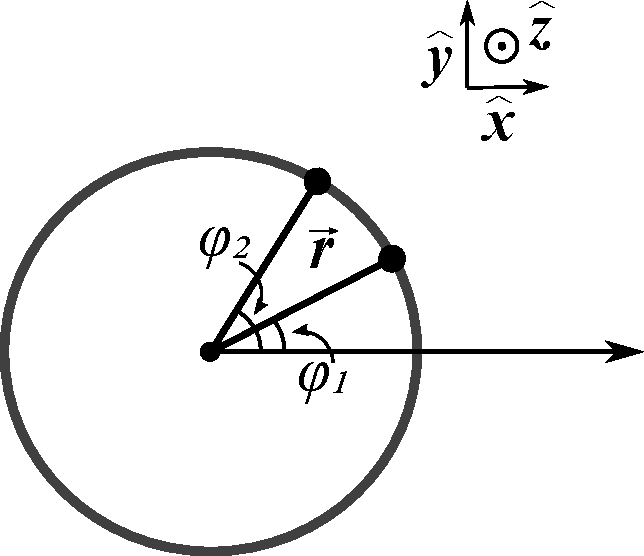
\includegraphics[width=.4\textwidth]{figurer/Roterende-Legeme}
\caption{Til to forskellige tider har det sorte punkt to forskellige vinkler med polæraksen (markeret med pil), der her er sammenfaldende med den kartesiske $x$-akse, mens legemet roterer om $z$-aksen. $\va{r}$ er en vektor fra origo til punktet, og har derfor længden $r$ og vinklen $\phi$ med polæraksen. Denne vektor ændrer sig i tid, som punktet flytter sig.}
\label{mek:fig:Roterende-Legeme}
\end{figure}
%
\cref{mek:fig:Roterende-Legeme} viser hvordan vinklen $\phi$ ændrer sig fra tidspunktet $t_1$ til $t_2$. Helt analogt til den translatoriske bevægelse defineres vinkelhastigheden, $\omega$, og vinkelacceleration, $\alpha$, som
%
\begin{equation}
    \omega\equiv\dot{\phi} \: , \qquad \alpha\equiv\dot{\omega}=\ddot{\phi} \: .
\end{equation}
%
Vinkelhastigheden er et udtryk for, hvor hurtigt et legeme roterer og har enheden $\si{\radian\per\second}$. Vinkelaccelerationen udtrykker, hvor hurtigt rotationshastigheden ændres i enheder af $\si{\radian\per\second\squared}$. Her er ''$\si{\radian}$``\;symbolet for enheden radianer.

\subsubsection{Inertimomentet}
Eksperimenter viser, at et legemes modstand mod acceleration ikke kun afhænger af legemets masse, men også placeringen af massen, hvorfor inertimomentet for et objekt defineres som\footnote{Symbolet $\equiv$ betyder indenfor fysik \textit{defineres som}, hvor $:=$ benyttes i matematik.}
%
\begin{equation} \label{mek:eq:Inertimoment}
    I \equiv \sum m_ir_i^2 \: ,
\end{equation}
%
hvor $m_i$ er massen af det $i$'te masseelement og $r_i$ er samme masseelements afstand til rotationsaksen. Ethvert legeme kan tænkes som bestående af en masse små dele, kaldet masseelementer, og inertimomentet udtrykker så hvor langt fra rotationsaksen et legemes masse er placeret. Definitionen er en smule rigid, men en konceptuel forståelse er tilstrækkelig her. $I$ afhænger af den akse, som legemet  roterer om, hvilket kan forklares ved at legemer lettere kan sættes i rotation om bestemte akser end andre. Dette kan man afprøve ved at tage et objekt og prøve at rotere det på forskellige måder. Man vil mærke at nogle rotationer er lettere end andre.


\subsection{Kinetisk Energi}
For translatorisk bevægelse defineres kinetisk energi som
%
\begin{equation} \label{mek:eq:Ktrans}
    K_{\text{trans}}=\frac{1}{2}mv_\textsc{cm}^2 \,,
\end{equation}
%
hvor $v_\textsc{cm}$ er massemidtpunktets fart. Hvis hele legemet bevæger sig med samme fart $v$ er $v_\textsc{cm} = v$, men hvis legemet eksempelvis roterer, bevæger forskellige dele af legemet sig med forskellige hastigheder. \\
Rotationskinetisk energi defineres tilsvarende som
%
\begin{equation} \label{mek:eq:Krot}
    K_{\text{rot}}=\frac{1}{2}I\omega^2 .
\end{equation}
%
Bemærk at \cref{mek:eq:Ktrans,mek:eq:Krot} har præcis sammen form, idet energien i begge tilfælde er proportional med en form for inerti og en fart i anden. Den totale kinetiske energi for et roterende legeme er summen af de to ovenstående
%
\begin{equation} \label{mek:eq:K}
    K_{\text{tot}}=K_{\text{trans}}+K_{\text{rot}} \: .
\end{equation}
%
At den totale kinetiske energi "bare"\;er summen af translatorisk og rotationel kinetisk energi, bør man strengt taget vise, men det er en smule omstændigt, hvorfor det undlades her.

\subsection{Dynamik}
%
\begin{figure}[h!]
\centering
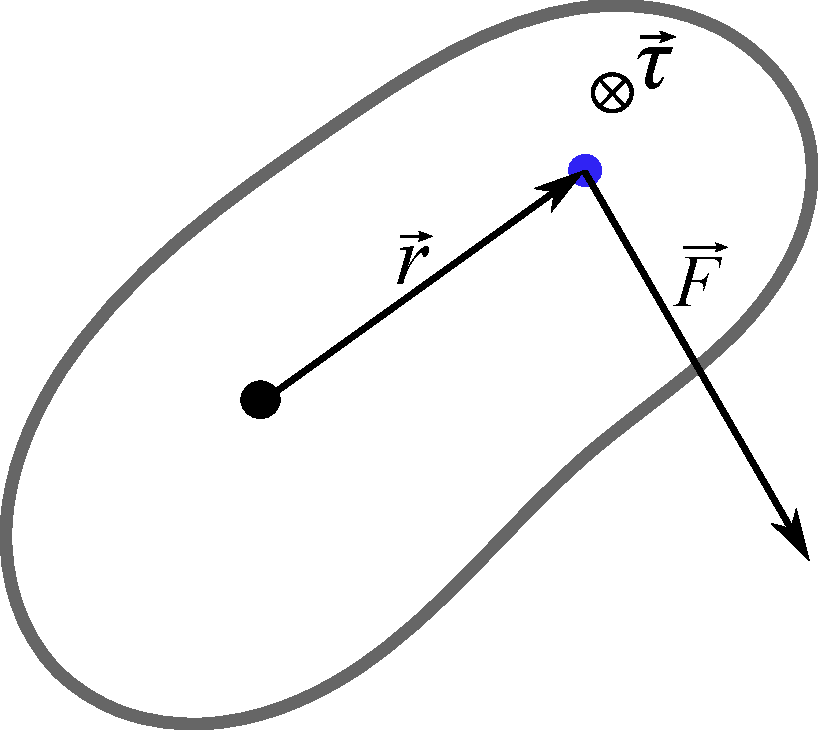
\includegraphics[width=.4\textwidth]{figurer/Kraftmoment}
\caption{En arbitrær kraft, $\va{F}$, virker i det blå punkt, hvorfor dette punkt kaldes kraftens angrebspunkt. Legemet roterer om en akse gennem det sorte punkt, der er ortogonal på tegningen. Det sorte punkt kan defineres som origo, hvorved vektoren fra rotationsaksen til kraftens angrebspunkt kaldes kraftens arm $\va{r}$. Kraftmomentet $\va{\tau}$ peger ind i tegningen, hvilket højrehåndsreglen viser.}
\label{mek:fig:Angrebspunkt}
\end{figure}
%
Kræfter er årsagen til bevægelse, som det kendes i fysik, og med hensyn til den translatoriske bevægelse er det ikke essentielt, hvor på legemet kraften virker, men det er det for rotationel bevægelse. Der findes mange dagligdags eksempler på dette, hvor et af de bedre er et værktøj, som en svensknøgle, der holder om en bolt. Jo længere nede på svensknøglen man holder, desto lettere er det at stramme eller løsne bolten. For at forstå fysikken bag dette, introduceres angrebspunktet for kraften $\va{F}$ som det punkt på et legeme, hvorpå kraften virker, se \cref{mek:fig:Angrebspunkt}. Yderligere defineres en vektor fra rotationsaksen til kraftens angrebspunkt, hvilket kaldes kraftens arm $\va{r}$. Herved kan kraftmomentet, $\va{\tau}$, defineres
%
\begin{equation} \label{mek:eq:Kraftmoment}
    \va{{\tau}} \equiv \va{r}\times\va{F} \: .
\end{equation}
%
Kraftmomentet er en vektor, der står ortogonalt på både kraften og dens arm, og den er parallel med rotationaksen. Kraftmomentets størrelse kan bestemmes som
%
\begin{equation} \label{mek:eq:KraftmomentNorm}
\tau = rF\sin\theta \: ,
\end{equation}
%
hvor $\theta$ er vinklen mellem $\va{r}$ og $\va{F}$. Dette leder til Newtons 2. lov for roterende legemer
\begin{align}
	\sum\tau = I\alpha \: .
\end{align}
Det ville være super anvendeligt, hvis dette galt ligeså alment, som Newtons 2. lov, $\sum\va{F} = m\va{a}$, men det er desværre ikke tilfældet. Den gælder for legemer, der er symmetriske omkring rotationsaksen og kun for størrelsen af vektorerne.